\documentclass[11pt]{article}
\usepackage{amsmath, amssymb}
\usepackage{geometry}
\geometry{margin=1in}
\usepackage{fancyhdr}
\usepackage{lastpage}
\usepackage{parskip} % Better paragraph spacing
\usepackage{titlesec} % Better section formatting
\usepackage{graphicx}
\usepackage{float}
\usepackage[most]{tcolorbox}
\usepackage{lmodern}
\usepackage{caption}
\usepackage{hyperref}
\usepackage{listings}
\usepackage{xcolor}
\usepackage{tikz}
\usetikzlibrary{automata, positioning, arrows.meta}

\definecolor{codegreen}{rgb}{0,0.6,0}
\definecolor{codegray}{rgb}{0.5,0.5,0.5}
\definecolor{codepurple}{rgb}{0.58,0,0.82}
\definecolor{backcolour}{rgb}{0.95,0.95,0.92}

% Define code styling
\lstdefinestyle{mystyle}{
    backgroundcolor=\color{backcolour},
    commentstyle=\color{codegreen},
    keywordstyle=\color{magenta},
    numberstyle=\tiny\color{codegray},
    stringstyle=\color{codepurple},
    basicstyle=\ttfamily\footnotesize,
    breakatwhitespace=false,
    breaklines=true,
    captionpos=b,
    keepspaces=true,
    numbers=left,
    numbersep=5pt,
    showspaces=false,
    showstringspaces=false,
    showtabs=false,
    tabsize=2
}

\lstset{style=mystyle}

% Define commands for reusable content
\newcommand{\coursename}{CS-550 - Formal Verification}
\newcommand{\lecturenum}{03}
\newcommand{\lecturedate}{\today}
\newcommand{\professor}{Viktor Kuncak}

\hypersetup{colorlinks=true,linkcolor=blue,urlcolor=blue}

% Configure section spacing
\titlespacing*{\section}{0pt}{2ex plus 1ex minus .2ex}{1.5ex plus .2ex}
\titlespacing*{\subsection}{0pt}{1.5ex plus 1ex minus .2ex}{1ex plus .2ex}
% Header / Footer
\pagestyle{fancy}
\fancyhf{}
\fancyhead[L]{\coursename}
\fancyhead[R]{Lecture \lecturenum}
\fancyfoot[L]{EPFL - Computer Science}
\fancyfoot[C]{Author: Jonathan Dutoit}
\fancyfoot[R]{Page \thepage\ of \pageref{LastPage}}

\begin{document}

\begin{center}
  {\large EPFL - Computer Science} \\[0.5em]
  {\Large \textbf{\coursename}} \\[0.5em]
  {\large Lecture \lecturenum\ --- \lecturedate} \\[0.5em]
  {\large Author: Jonathan Dutoit} \\[0.5em]
  {\large Professor: \professor} \\[0.5em]
\end{center}

\vspace{0.5cm}

\begin{center}
  {\LARGE \textbf{Formal Proofs}}
\end{center}

\vspace{0.5cm}

\subsection*{Formal Proof System}

We will consider some set of logical formulas \textit{F} (e.g., propositional logic)

\begin{tcolorbox}[
    enhanced,
    frame hidden,
    borderline west={2pt}{0pt}{black},
    boxsep=5pt,
    left=8pt
]
\textbf{Definition.} An proof system is (\textit{F, Infer}) where Infer $\subseteq F^{*} \times F$ a decidable set of \textit{inference} steps. 
\begin{itemize}
	\item a set is \textit{decidable} iff there is a program to check if an element belongs to it
	\item given a set \textit{S}, notation $S^{*}$ denotes all finite sequences with elements from \textit{S} \\
\end{itemize}

We schematically write an inference step $((P_1, ..., P_n), C) \in \text{Infer}$ by $$\frac{P_1 ... P_n}{C}$$ 

and we say that from $P_1, ..., P_n$ (\textbf{premises}) we derive \textit{C} (\textbf{conclusion}). \\

An inference step is called an \textit{axiom} instance when $n = 0$ (it has no premises). 

\end{tcolorbox}

\begin{tcolorbox}[
    enhanced,
    frame hidden,
    borderline west={2pt}{0pt}{black},
    boxsep=5pt,
    left=8pt
]
\textbf{Definition.} Given (\textit{F}, Infer) where Infer $\subseteq F^{*} \times F$. \\ 

We define a \textbf{proof} in (\textit{F}, Infer) as a finite sequence of inference steps $S_0, ..., S_m \in$ Infer such that, for each $S_i$ where $0 \leq i \leq m$, for each premise $P_j$ of $S_i$ there exists $0 \leq k < i$ such that $P_j$ is the conclusion of $S_k$.
\[
	\begin{align*}
		S_0 : &\ ((), &\ C_0) \\
		      &\ ... &\ \\
		S_k : &\ ((........), &\ \mathbf{P_j}) \\ 
		      &\ ... &\ \\
		S_i : &\ ((..., \mathbf{P_j}, ...), &\ C_i)
	\end{align*}
.\] 
Given the definition of the proof, we can replace each premise $P_j$ with the index \textit{k} where $P_j$ was the conclusion of $S_k$ $(P_j \equiv \text{Conc}(S_k))$ \\

A proof is then a sequence of elements from $\{0, 1, ...\}* \times F$ where each $S_i$ in the sequence is of form $(k_1, ..., k_n, C)$ for $0 \leq k_1, ..., k_n < i$ and where (Conc($S_{k_1}$), ..., Conc($S_{k_n}$), C) $\in$ Infer. \\

This is possible since we can reduce premises to axioms. 
\end{tcolorbox}
\begin{figure}[H]
    \centering
    \begin{tikzpicture}[
        >=Stealth,
        font=\small,
        % Styles
        formula/.style={
            circle,
            draw=blue!55!black,
            fill=blue!8,
            line width=0.8pt,
            minimum size=11mm,
            inner sep=2pt
        },
        axiom/.style={
            formula,
            draw=green!45!black,
            fill=green!12
        },
        inference/.style={
            formula,
            draw=blue!55!black,
            fill=blue!8
        },
        dependency/.style={
            ->,
            thick,
            draw=black!80
        },
        step/.style={
            font=\scriptsize,
            align=center,
            inner sep=2pt
        }
    ]

    % Final inference
    \node[inference] (Cm) at (0,3.8) {$C_m$};
    \node[step] at (0,4.55) {$S_m$\\: Conclusion};

    % Intermediate inferences
    \node[inference] (Ci) at (-2,2) {$C_i$};
    \node[inference] (Cj) at ( 2,2) {$C_j$};

    \node[step] at (-2,1.10) {$S_i$};
    \node[step] at ( 2,1.10) {$S_j$};

    % Axiom conclusions
    \node[axiom] (A0) at (-3.3,0) {$A_0$};
    \node[axiom] (A1) at (-1.1,0) {$A_1$};
    \node[axiom] (A2) at ( 1.1,0) {$A_2$};
    \node[axiom] (A3) at ( 3.3,0) {$A_3$};

    % ------------------------------------------------
    % Dependencies: premise conclusion -> new conclusion
    % ------------------------------------------------

    \draw[dependency] (A0) -- (Ci);
    \draw[dependency] (A1) -- (Ci);

    \draw[dependency] (A2) -- (Cj);
    \draw[dependency] (A3) -- (Cj);

    \draw[dependency] (Ci) -- (Cm);
    \draw[dependency] (Cj) -- (Cm);

    % ------------------------------------------------
    % Legend
    % ------------------------------------------------

    \begin{scope}[shift={(4.4,2.8)}]
        \draw[rounded corners=2pt, draw=black!35]
            (0,0) rectangle (5,1.65);

        \node[axiom, minimum size=6mm]
            (legendA) at (0.45,1.25) {};
        \node[anchor=west, align=left]
            at (0.9,1.25) {Axiom (no premises)};

        \node[inference, minimum size=6mm]
            (legendI) at (0.45,0.7) {};
        \node[anchor=west, align=left]
            at (0.9,0.7) {Inference conclusion};

        \draw[dependency] (0.15,0.2) -- (0.75,0.2);
        \node[anchor=west, align=left]
            at (0.9,0.2) {Premise dependency};
    \end{scope}
    \end{tikzpicture}

    \caption{A proof as a directed acyclic graph (DAG). Each node
    represents the conclusion of an inference step, and each arrow
    represents a premise dependency.}
    \label{fig:proof_dag_clean}
\end{figure}

To check such proof, for each node, follow all its incoming edges backwards in the order of their indices to find the premises, then check that the inference steps in in Infer. 

\subsection*{A Minimal Propositional Logic Proof System}

Formulas \textit{F} defined by $F ::= x \, | \, 0 \, | \, F \to F$

Shorthand: \\
$\neg F \equiv F \to 0$

Inference rules: Infer = $P_2 \cup P_3 \cup MP$ where:
\[
	\begin{array}{l l l l l}
		P_2 & = & \{((), & F \to (G \to F) & ) \, | \, F, G \in F\} \\ 
		P_3 & = & \{((), & ((F \to (G \to H)) \to ((F \to G) \to (F \to H)) & ) \, | \, F, G, H \in F\} \\ 
		MP & = & \{((F \to G, F), & G & ) \, | \, F, G \in F\}
	\end{array}
.\] 

Elements of $P_1, P_2, P_3$ are all axioms. These are infinite sets, but are given a schematic way and there is an algorithm to check if a given formula satisfies each of the schemas. 


\textbf{Exercise:} proof of $a \to a$

Proof system: 
\[
	P_2 : F \to (G \to F) \quad \quad P_3 : ((F \to (G \to H)) \to ((F \to G) \to (F \to H)) \quad \quad MP : \frac{F \to G, F}{G} 

	\text{We start by assuming} F \leftrightarrow a, \, G \leftrightarrow (a \to a), \, H \leftrightarrow a

	\begin{array}{l l l}
		1. & (a \to ((a \to a) \to a)) \to ((a \to (a \to a)) \to (a \to a)) & \text{Instance of } P_3 \\
		2. & (a \to ((a \to a) \to a) & \text{Instance of } P_2\\
		3. & (a \to (a \to a)) \to (a \to a) & \text{MP on 1 and 2} \\ 
		4. & a \to (a \to a) & \text{Instance of } P_2 \\
		5. & a \to a & \text{MP on 3 and 4} 
	\end{array}
\] 

\begin{figure}[H]
    \centering
    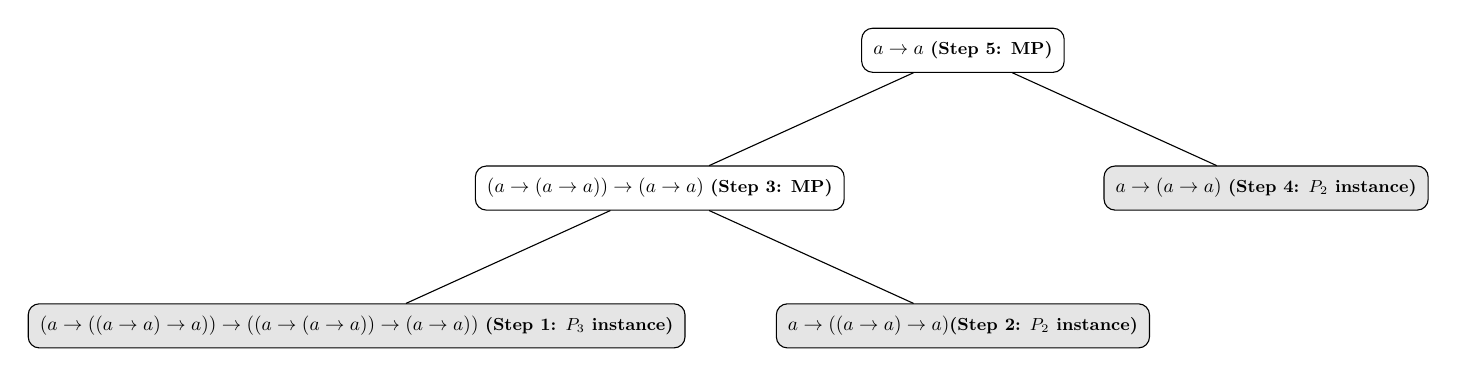
\begin{tikzpicture}[
        scale=0.7,
        transform shape,
        every node/.style={rectangle, draw, rounded corners, minimum height=8mm, inner sep=6pt, fill=white},
        >=Stealth,
        level distance=2.5cm,
        sibling distance=11cm
    ]
        % Root: Final conclusion a -> a (Derived via MP on lines 3 and 4)
        \node {$a \to a$ \small{\textbf{(Step 5: MP)}}}
            % Child 1: Line 3 premise ((a -> (a -> a)) -> (a -> a))
            child { node {($a \to (a \to a)) \to (a \to a)$ \small{\textbf{(Step 3: MP)}}}
                % Leaves / Sub-proof parts
                child { node[fill=gray!20] {$(a \to ((a \to a) \to a)) \to ((a \to (a \to a)) \to (a \to a))$ \small{\textbf{(Step 1: $P_3$ instance)}}} }
		child { node[fill=gray!20] {$a \to ((a \to a) \to a) $\small{\textbf{(Step 2: $P_2$ instance)}}} }
            }
            % Child 2: Line 4 premise (a -> (a -> a))
	    child { node[fill=gray!20] {$a \to (a \to a)$ \small{\textbf{(Step 4: $P_2$ instance)}}} };

    \end{tikzpicture}
    \caption{DAG proof structure for $a \to a$ using Modus Ponens (MP) and axiom instances $P_2$ and $P_3$.}
\end{figure}

\section*{Soundness of a Proof System}

\begin{tcolorbox}[
    enhanced,
    frame hidden,
    borderline west={2pt}{0pt}{black},
    boxsep=5pt,
    left=8pt
]
\textbf{Definition.} Given (\textit{F}, Infer), Infer $\subseteq F^{*} \times F$ \textbf{and a set of assumptions} $A \subseteq F$, a \textbf{derivation from} \textit{A} in (\textit{F}, Infer) is a proof in (\textit{F}, infer') where: $$ \text{Infer}' = \text{Infer} \cup \{((), F) \, | \, F \in A\}$$ 
Thus, assumptions from \textit{A} are treated just as axioms. \emph{Hence, A expands the proof system by treating every formula in A as an extra axiom (i.e, a premise-free rule that can be introduced at any point in the proof).}
\end{tcolorbox}

\begin{tcolorbox}[
    enhanced,
    frame hidden,
    borderline west={2pt}{0pt}{black},
    boxsep=5pt,
    left=8pt
]
\textbf{Definition.} We say that $F \in F$ is provable from assumptions \textit{A}, denote $\vdash_{\text{Infer}} F$ iff there exists a derivation from \textit{A} in Infer that contains an inference step whose conclusion is \textit{F}. \\

We write $\vdash_{\text{Infer}} F$ to denote that there exists a proof in Infer containing \textit{F} as a conclusion (same as $\varnothing \vdash_{\text{Infer}} F$).  \\

\emph{This is syntactic process. It relies purely on symbol manipulation and matching rules, without caring about what the symbols actually mean. It means that the formula F can be mechanically derived using the proof system's inference rules.}
\end{tcolorbox}

\begin{tcolorbox}[
    enhanced,
    frame hidden,
    borderline west={2pt}{0pt}{black},
    boxsep=5pt,
    left=8pt
]
\textbf{Definition.}  Given a set $A \subseteq F$ where \textit{F} are in propositional logic, and $C \in F$, we say that \textit{C} is a \textbf{semantic consequence} of \textit{A}, denote $A \models C$ iff for every environment \textit{e} that defines all variables in $FV(C) \cup \bigcup_{P \in A} FV(P) $ if $[\![P]\!]_e = 1$ for all $P \in A$, then $[\![C]\!]_e = 1$. \\ 

$A \models C$ means the conclusion is guaranteed to be true whenever the premises are true. In other words, there is not counterexample where all premises are true and the conclusion is false. 
\end{tcolorbox}

\begin{tcolorbox}[
    enhanced,
    frame hidden,
    borderline west={2pt}{0pt}{black},
    boxsep=5pt,
    left=8pt
]
\textbf{Definition.} Given (\textit{F}, Infer) where \textit{F} are propositional, step $((P_1...P_n), C) \in$ Infer is \textbf{sound} iff $\{P_1, ..., P_n\} \models C$. Proof system Infer is sound if every inference step is sound. \\

For axioms, this definition reduces to saying that \textit{C} is true for all interpretations, i.e, that \textit{C} is a valid formula (tautology). 
\end{tcolorbox}

\begin{tcolorbox}[
    enhanced,
    frame hidden,
    borderline west={2pt}{0pt}{black},
    boxsep=5pt,
    left=8pt
]
\textbf{Definition.} Let (\textit{F}, Infer) where \textit{F} are propositional logic formulas. If every inference rule in Infer is sound, then $A \vdash_{\text{Infer}} F$ implies $A \models F$. \\

Proof is immediate by induction on the length of the formal proof. \\
Consequence: $\vdash_{\text{Infer}} F$ implies \textit{F} is a tautology. 
\end{tcolorbox}

\subsection*{Semantic vs Syntactic Consequence}
\textbf{Semantic consequence}: We check whether $\{ A_1 \} \models G$ by checking all possible interpretations: in every propositional assignment (any "world" we can imagine) if $A_1$ is true, then so if G. For propositional logic, a world gives truth values (0 or 1) for the variables. 

\textbf{Syntactic consequence (provability)}: We check whether $\{ A_1 \} \vdash G$ by finding a derivation of \textit{G} with $A_1$ as an additional axiom. Syntactic consequence is specific for a particular proof system. 

In general we have a set of assumptions, $A = \{A_1, A_2, ...\}$

For a given proof system, we have two possible conclusions:
\begin{itemize}
	\item soundness: if $A \vdash G$, then $A \models G$ \\
	(without this, our proof system is "broken")
	\item completeness: if $A \models G$, then $A \vdash G$ \\
	(without this, there are true things we cannot prove, which may be OK)
\end{itemize}

\subsection*{Completeness}

\begin{tcolorbox}[
    enhanced,
    frame hidden,
    borderline west={2pt}{0pt}{black},
    boxsep=5pt,
    left=8pt
]
\textbf{Definition.} A proof system is \textbf{complete} if it derives all formulas we want it to derive. Completeness for classical propositional logic means that the system derives all propositional tautologies.\emph{Meaning every tautology can be proven using these rules}.

\end{tcolorbox}

\textbf{Example: } Is our example system complete with respect to formulas built from $to$ and $0$? $$  P_2 : F \to (G \to F) \quad \quad P_3 : ((F \to (G \to H)) \to ((F \to G) \to (F \to H)) \quad \quad MP : \frac{F \to G, F}{G} $$ 

\begin{itemize}
	\item In particular, if we are given an arbitrary valid propositional formula (propositional tautology), is there always a way to derive it using the axioms and the MP rule? 
	\item Does there exist a tautology that is not reachable from axioms using MP rule?
	\item Is valid formula $ 0 \to a$ provable? 
\end{itemize}

The axioms don't say anything about the $0$ constant. It is as if it was any other subformula. Take proof: 
\[
	\begin{array}{l}
	... \\
	a \to a\\ 
	(a \to a) \to (0 \to (a \to a)) \quad (\text{Axiom}) \\
	0 \to (a \to a) \quad (\text{MP})
	\end{array}
.\] 

Replace 0 with e.g., $b \to c$ in the proof above. It will get a valid proof: 
\[
	\begin{array}{l}
		... \\
		a \to a \\ 
		(a \to a) \to ((b \to c) \to (a \to a)) \quad (\text{Axiom}) \\ 
		(b \to c) \to (a \to a) \quad (\text{MP})
	\end{array}
.\] 

Replacing 0 with some fixed formula gives us valid proofs. 

Now let's suppose that our proof system can prove $0 \to a$. Then it can also prove a formula resulting by $0$ with $a \to a$, so there would exists a proof of $(a \to a) \to a$. 
We have shown before that we can derive $a \to a$, so we would also derive $a$ using MP. But $a$ is not a tautology, which is a contradiction with the fact that the system is sound. 

\textbf{Note:} The Sheffer Stroke which represents the NAND operator has properties: 
\begin{itemize}
	\item \textbf{Functional completeness}: can express any truth table on its own, i.e, it build all other logical connectives (like AND, OR, NOT, IMPLIES). 
	\item \textbf{Deductive completeness}: Once properly formulated into an axiomatic system, a Sheffer stroke proof system is deductively complete for classical propositional logic. Every tautology can be successfully derived using its rules.
\end{itemize}

\section*{Towards Propositional Resolution}

Consider propositional formulas with $\land, \lor, \neg$ 

\textbf{Case analysis proof rule.} $\{((F, G), F[x := 0] \lor G[x := 1]) \, | \, F, G \in F, x - \text{variable}\}$:
\[
	\frac{F \quad \quad \quad \quad G}{F[x := 0] \lor G[x := 1] }
.\] 

Proof of soundness. To show $\{F, G\} \models (F[x := 0] \lor G[x := 1])$, consider an environment \textit{e} and assume $[\![F]\!]_e = 1$ and $[\![G]\!]_e = 1$. 
\begin{itemize}
	\item If \textit{e(x) = 0}, then $[\![F[x := 0]]\!]_e = [\![F]\!]_e = 1$, so the first disjunct is 1. 
	\item If \textit{e(x) = 1}, then $[\![G[x := 1]]\!]_e = [\![G]\!]_e = 1$, so the second disjunct is 1. 
\end{itemize}
In both cases, the disjunction evaluates to 1 in \textit{e}.

\textbf{Simplification rules} that preserve equivalence: $0 \land F \rightsquigarrow 0$, $F \land 0 \rightsquigarrow 0$, $ 1 \land F \rightsquigarrow F$, $F \land 1 \rightsquigarrow F$, $0 \lor F \rightsquigarrow F$, $F \lor 0 \rightsquigarrow F$, $1 \lor F \rightsquigarrow 1$, $F \lor 1 \rightsquigarrow 1$, $\neg 0 \rightsquigarrow 1$, $\neg 1 \rightsquigarrow 0$.  

Introduce inferences $\{((F), F') \, | \, F' \, \text{ is simplified} \, F\}$. These rules are also sound. Let Infer$_D$ be the proof system with the above case analysis and simplification rules.  

\textbf{Example Derivation} from $A = \{a \land b, \neg b \lor \neg a\}$. We want to show $A \vdash 0$. This is called proof by refutation. In automated reasoning, formal verification, and SAT solvers, showing that a set of assumptions leads to 0 is one of the most powerful techniques available, known as refutation or \textbf{proof by contradiction}.  

Actually, the assumptions in $A$ are completely \textcolor{blue}{unsatisfiable}. There is no possible truth assignment (world) where all formulas in A can be true at the same time.

\textit{A} naturally leads to a contradiction:
\begin{itemize}
	\item Assumption 1 $a \land b$: Tells you that both $a$ is true and $b$ is true.
	\item Assumption 2 $\neg b \lor \neg a \equiv \neg(a \land b)$  (De Morgan's laws) tells that it is not the case that both are true.
\end{itemize}

Using inference rules (\textit{case analysis} or \textit{resolution rules}, the system clashes these opposing facts until everything cancels out, leaving you with 0.

The \textbf{ultimate "success" state} of a resolution algorithm is deriving the empty clause (0). Deriving 0 acts as a certificate proving that your initial set of constraints or code specifications contains a bug, a dead end, or a logical contradiction.

\begin{tcolorbox}[
    enhanced,
    frame hidden,
    borderline west={2pt}{0pt}{black},
    boxsep=5pt,
    left=8pt
]
\textbf{Definition.} A \textit{set A} of formulas is \textit{satisfiable} if there exists \textit{e} such that, for every $F \in A, [\![F]\!]_e = 1$ \\

When $A = \{F_1, ..., F_n\}$ (finite), the notion is the same as the satisfiability of $F_1 \land ... \land F_n$. \\ 

Otherwise, we call the set \textit{A unsatisfiable}. 
\end{tcolorbox}

\textcolor{blue}{Theorem (Soundness Consequence)} \\
\noindent
\vrule width 1pt
\hspace{0.5em}
\begin{minipage}{0.9\textwidth}
\vspace{0.3cm}
\textit{If} $A \vdash_{\text{Infer}_D} 0$ \textit{then A is unsatisfiable}.  \\

If there exists \textit{e} such that \textit{e(F) = 1} for all $F \in A$ then by soundness of Infer$_D$, \textit{e(0) = 1}, a contradiction. So there is no such \textit{e}.
\end{minipage}

\textcolor{blue}{Theorem (Refutation Completeness)} \\ 
\noindent
\vrule width 1pt
\hspace{0.5em}
\begin{minipage}{0.9\textwidth}
\vspace{0.3cm}
\textit{If a finite set A is unsatisfiable}, then $A \vdash_{\text{Infer}_D} 0$ \\ 

Proof hint: take conjunction of formulas in \textit{A} and existentially quantify it to get \textit{A'}. \\
What is the relationship of the truth of \textit{A'} and the satisfiability of A? For a conjunction for formulas \textit{F}, can you express $\existsx. F$ using Infer$_D$?
\end{minipage}

\textbf{Illustration of completeness}: Let $A = \{F_1, F_2\}$ and let $FV(F_1) \cup FV(F_2) = \{x_1, ..., x_n\}$ and let \textit{x} be some $x_i$. We have the following equivalences: 
\[
\begin{align*}
    &\exists x.(F_1 \land F_2) \\
    \equiv\ & (F_1 \land F_2)[x := 0] \lor (F_1 \land F_2)[x := 1] \\
    \equiv\ & (F_1[x := 0] \land F_2[x := 0]) \lor (F_1[x := 1] \land F_2[x := 1]) \\
    \equiv\ & (F_1[x := 0] \lor F_1[x := 1]) \land (F_1[x := 0] \lor F_2[x := 1]) \land \\
            & (F_2[x := 0] \lor F_1[x := 1]) \land (F_2[x := 0] \lor F_2[x := 1])
\end{align*}
.\] 

Where we try both values meaning of substitution. This is like doing the \underline{case analysis}. 

Existentially quantifying over a variable gives us result of applying decision rule to all pairs of formulas $F_1, F_2$. 

Systematically applying rules will derive formula \textit{Z} equivalent to $\exists x_1. ... \exists x_n. (F_1 \land F_2). $

When \textit{A} is unsatisfiable, \textit{Z} is equivalent to 0, and has no variables. By simplification rules, we can derive 0.  

\vspace{0.5cm}

\begin{center}
  {\LARGE \textbf{Resolution on Clauses}} \\
	\vspace{0.25cm}
  \small{We previously considered a "simple" proof system that's easy to understand. In practice, we often don't work with arbitrary formulas, but with clauses since they can be represented more efficiently.}
\end{center}
\vspace{0.5cm}

\begin{tcolorbox}[
    enhanced,
    frame hidden,
    borderline west={2pt}{0pt}{black},
    boxsep=5pt,
    left=8pt
]
\textbf{Definitions}
\begin{itemize}
	\item A propositional \textbf{\textit{literal}} is either a variable (e.g., \textit{s}) or its negation ($\neg x$). 
	\item A \textbf{\textit{clause}} is a disjunction of literals. \\
	For convenience, we can represent clause as a finite \textit{set of literals} (because of associativity, commutativity, and idempotence of $\lor$). 
\end{itemize}
\end{tcolorbox}

If \textit{C} is a clause then $[\![C]\!]_e = 1$ iff there exists a literal $L \in C$ such that $[\![L]\!]_e = 1$. 

We represent 0 using the empty clause $\varnothing$ (represents \textbf{contradiction})

As for any formulas, a finite set of clauses \textit{A} can be interpreted as a conjunction. Thus, a set of clauses can be viewed as a formula in conjunctive normal form: $$A = \{\{a\}, \{b\}, \{\neg a, \neg b\}\}$$ represents the formula $$ a \land b \land (\neg a \lor \neg b) $$

\begin{figure}[H]
    \centering
    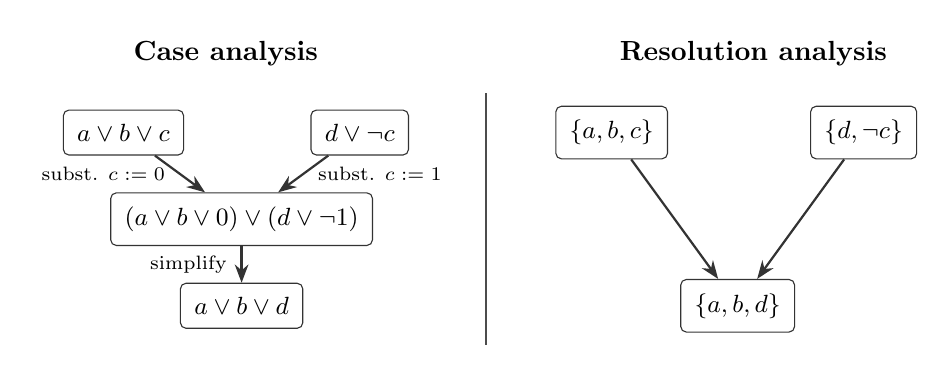
\begin{tikzpicture}[
        >=Stealth,
        font=\small,
        every node/.style={
            rectangle,
            draw=black!80,
            rounded corners=2pt,
            inner sep=5pt,
            fill=white
        },
        dependency/.style={
            ->,
            thick,
            draw=black!80
        }
    ]
        % ------------------------------------------------
	% Titles above each side (no border/fill)
        % ------------------------------------------------
        \node[draw=none, fill=none, font=\bfseries] at (-1.5, 3.2) {Case analysis};
        \node[draw=none, fill=none, font=\bfseries] at (5.2, 3.2) {Resolution analysis};
        % ------------------------------------------------
        % Left Side: Formulas with Substitutions
        % ------------------------------------------------
        \node (L1) at (-2.8, 2.2) {$a \lor b \lor c$};
        \node (L2) at (0.2, 2.2) {$d \lor \neg c$};
        \node (L3) at (-1.3, 1.1) {$(a \lor b \lor 0) \lor (d \lor \neg 1)$};
        \node (L4) at (-1.3, 0.0) {$a \lor b \lor d$};

        % Left side dependency arrows
	\draw[dependency] (L1) -- (L3) node[midway, left, draw=none, fill=none, font=\scriptsize] {subst. $c:=0$};
        \draw[dependency] (L2) -- (L3) node[midway, right, draw=none, fill=none, font=\scriptsize] {subst. $c:=1$};
        \draw[dependency] (L3) -- (L4) node[midway, left, draw=none, fill=none, font=\scriptsize] {simplify};
        % ------------------------------------------------
        % Vertical Dividing Line
        % ------------------------------------------------
        \draw[thick, draw=black!70] (1.8, 2.7) -- (1.8, -0.5);

        % ------------------------------------------------
        % Right Side: Clause Sets (Resolution)
        % ------------------------------------------------
        \node (R1) at (3.4, 2.2) {$\{a, b, c\}$};
        \node (R2) at (6.6, 2.2) {$\{d, \neg c\}$};
        \node (R3) at (5.0, 0.0) {$\{a, b, d\}$};

        % Right side dependency arrows
        \draw[dependency] (R1) -- (R3);
        \draw[dependency] (R2) -- (R3);

    \end{tikzpicture}
    \label{fig:resolution_clauses}
\end{figure}

Clausal resolution rule (decision rule for clauses): 
$$\frac{C_1 \cup \{x\} \quad \quad C_2 \cup \{\neg x \}}{C_1 \cup C_2}$$

\textcolor{blue}{Theorem (Soundness)} \\
\noindent
\vrule width 1pt
\hspace{0.5em}
\begin{minipage}{0.9\textwidth}
\vspace{0.3cm}
\textit{Clausal resolution is sound: for all clauses} $C_1, C_2$ \textit{and propositional variable x}, \\
$\{C_1 \cup \{x\}, C_2 \cup \{\neg x\}\} \models C_1 \cup C_2$
\end{minipage}

\textcolor{blue}{Theorem (Refutational Completeness)} \\ 
\noindent
\vrule width 1pt
\hspace{0.5em}
\begin{minipage}{0.9\textwidth}
\vspace{0.3cm}
\textit{A finite set of clauses A is unsatisfiable if and only if there exists a derivation of the empty clause from A using clausal resolution}. 
\end{minipage}

\textbf{Example:} Use resolution to prove that the following formula is valid: $$\neg(a \land b \land (\neg a \lor \neg b))$$ Prove that its negation is unsatisfiable set of clauses: 

\begin{figure}[H]
    \centering
    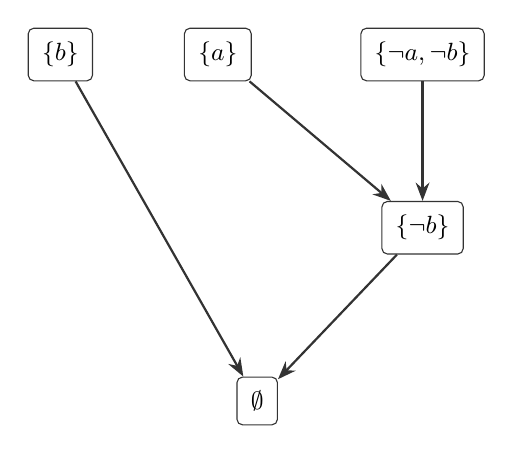
\begin{tikzpicture}[
        >=Stealth,
        font=\small,
        every node/.style={
            rectangle,
            draw=black!80,
            rounded corners=2pt,
            inner sep=5pt,
            fill=white
        },
        dependency/.style={
            ->,
            thick,
            draw=black!80
        }
    ]
        \node (R2) at (2, 2.2) {$\{b\}$};
        \node (R1) at (4, 2.2) {$\{a\}$};
        \node (R3) at (6.6, 2.2) {$\{\neg a,\neg b\}$};
        \node (R4) at (6.6, 0) {$\{\neg b\}$};
        \node (R5) at (4.5, -2.2) {$\emptyset$};

        % Right side dependency arrows
        \draw[dependency] (R1) -- (R4);
        \draw[dependency] (R3) -- (R4);
	
        \draw[dependency] (R4) -- (R5);
        \draw[dependency] (R2) -- (R5);
    	\end{tikzpicture}
\end{figure}

\subsection*{Unit Resolution}

\begin{tcolorbox}[
    enhanced,
    frame hidden,
    borderline west={2pt}{0pt}{black},
    boxsep=5pt,
    left=8pt
]
\textbf{Definition.} A \textit{unit clause} is a clause that has precisely one literal; it's of the form $\{L\}$ \\
Given a literal \textit{L}, its complement $\bar{L}$ is defined by $\bar{x} = \neg x, \quad \overline{\neg x} = x$. \\

\textbf{Unit resolution} is a special case of resolution where at least one of the clauses is a unit clause: $$\frac{C \quad \quad \{L\}}{C \setminus \{\bar{L}\}}$$

Soundness: if \textit{L} is true, then $\bar{L}$ is false, so it can be deleted from a disjunction \textit{C}.
\end{tcolorbox}

\emph{Subsumption}: when applying resolution, if we obtain a clause \textit{C'} $\subseteq$ \textit{C} that is subset of a previously derived one, we can delete \textit{C} so we do not consider it any more. Any use of \textit{C} can be replaced by use of \textit{C'} with progress towards $\emptyset$ at least as good. 

\textbf{Conclusion}: if we derive $\{L\}$ we can remove all other occurrences of \textit{L} and $\bar{L}$: if $L \in C$ then \textit{C} is subsumed by $\{L\}$ and if $\bar{L} \in C$ then \textit{C} is subsumed by $C \setminus \{\bar{L}\}$. 

\vspace{0.5cm}

\begin{center}
  {\LARGE \textbf{From Formulas to Clauses}}
\end{center}
\vspace{0.5cm}

\subsection*{Normal Form Transformation}

Transformation of an arbitrary formula into a set of clauses is exponential in general, applying from left to right equivalence $$F_1 \land (F_2 \land F_3) \leftrightarrow (F_1 \lor F_2) \land (F_1 \lor F_3)$$ duplicates sub-formulas $F_1$, which may result in an exponential larger formula if for instance $F_1$ is not a propositional variable. 

\textbf{Key idea}: Transform formula into \textit{disjunctive} normal form, because checking satisfiability of formula in disjunctive normal form is trivial, such formula is a disjunction of conjunctions $D_i$ and we have these equivalences: 

\[
	\begin{gathered}
		\exists e. [\![D_1 \lor ... \lor D_n]\!]_e = 1 \\
		\exists e.([\![D_1]\!]_e == 1 \lor ... \lor [\![D_n]\!]_e = 1) \\
		 (\exists e. [\![D_1]\!]_e = 1) \lor  ... \lor (\exists e. [\![D_n]\!]_e = 1)
	\end{gathered}
.\] 

and the last condition is trivial to check, because we check satisfiability of conjunction $D_i$ separately. 

\begin{tcolorbox}[
    enhanced,
    frame hidden,
    borderline west={2pt}{0pt}{black},
    boxsep=5pt,
    left=8pt
]
\textbf{Definition.} Formula $F_1$ and $F_2$ are \textbf{equivalent} iff: $F_1 \models F_2$ and $F_2 \models F_1$ ($\forall e. [\![F_1]\!]_e = [\![F_2]\!]_e$) 
\end{tcolorbox}

\begin{tcolorbox}[
    enhanced,
    frame hidden,
    borderline west={2pt}{0pt}{black},
    boxsep=5pt,
    left=8pt
]
\textbf{Definition.} Formulas $F_1$ and $F_2$ are \textbf{equisatisfiable} iff: $F_1$ is satisfiable whenever $F_2$ is satisfiable. 
\end{tcolorbox}

\textbf{Note}: Equivalent formulas are always equisatisfiable, but the converse is not the case in general. 

\textbf{Example:} consider these two formulas: $$F_1: (a \land b) \lor c \quad \quad \quad F_2: (x \leftrightarrow (a \land b)) \land (x \lor c)$$

They are equisatisfiable but not equivalent. For example, given $e = \{(a, 1), (b, 1), (c, 0), (x, 0)\}, [\![F_1]\!]_e = 1$ whereas $[\![F_2]\!]_e = 0$. Interestingly, every choice of $a, b, c$ that makes $F_1$ true can be extended to make $F_2$ true appropriately, if we chose $x$ as $[\![a \land b]\!]_e$. 

\subsection*{Flatenning as Satisfiability Preserving Transformation}

\textit{Observation}: Let $F$ be a formula, $G$ another formula, and $x \notin FV(F)$ a propositional variable. Let $F[G := x]$ denote the result of replacing an occurrence of formula \textit{G} inside \textit{F} with \textit{x}. Then \textit{F} is equisatisfiable with $$(x = G) \land F[G := x]$$ where $=$ denotes $\leftrightarrow$. 

\emph{Strategy}: apply transformation from smallest non-variable subformulas. \textbf{Tseytin's Transformation}!  

Consider formula with $\neg, \land, \lor, \to, =, \oplus$ 
\begin{itemize}
	\item Replace $F_1 \to F_2$ with $\neg F_1 \lor F_2$ and push negation into the propositional variables using De Morgan's laws and switching between $\oplus$ and $=$. 
	\item Repeat: flatten an occurrence of a binary connective whose arguments are literals
	\item In the resulting conjunction, express each equivalence as a conjunction of clauses: 
\end{itemize}

\[
	\begin{array}{l |  l}
		\text{conjunct} & \text{corresponding clauses} \\
		 & \\
		x = (a \land b) & \Leftrightarrow (x \to (a \land b)) \land ((a \land b) \to x) \\
		 & \Leftrightarrow (\neg x \lor (a \land b)) \land (\neg(a \land b) \lor x) \\
		  & \Leftrightarrow (\neg x \lor a) \land (\neg x \lor b) \land (\neg a \lor \neg b \lor x) \\ 
		 & \{\bar{x}, a\}, \{\bar{x}, b\}, \{\bar{a}, \bar{b}, x\} \\ 
		 & \\
		x = (a \lor b) & \{\bar{x}, a, b\}, \{\bar{a}, x\}, \{\bar{b}, x\}

		& \\ 
		x = (a = b) & \Leftrightarrow (x \to (a = b)) \land ((a = b) \to x) \\ 
		 & \Leftrightarrow (\neg x \lor ((a \to b) \land (b \to a)) \land (\neg ((a \to b) \land (b \to a)) \lor x) \\ 
		 & \Leftrightarrow (\neg x \lor ((\neg a \lor b) \land (a \lor \neg b)) \land (\neg ((\neg a \lor b) \land (a \lor \neg b)) \lor x) \\
		 & \{\bar{x}, \bar{a}, b \}, \{\bar{x}, a, \bar{b} \}, \{x, a, b\}, \{x, \bar{a}, \bar{b}\} \\
	\end{array}
\] 

\textbf{Example}: Find an Equisatisfiable Set of Formulas in CNF 
$$
\begin{array}{l}
	\{\boxed{c \land a} \lor (\neg c \land b) \} \\ [1em]
	\{ x_1 \lor \boxed{\neg c \land b}, \ x_1 \leftrightarrow (c \land a) \}\\[1em]

\{ x_1 \lor x_2, \ x_2 \leftrightarrow (\neg c \land b),  \\
\quad x_1 \leftrightarrow (c \land a) \} & \\[1em]

\{ x_1 \lor x_2, \ x_2 \to (\neg c \land b), \ (\neg c \land b) \to x_2, \\
\quad x_1 \to (c \land a), \ (c \land a) \to x_1 \} & \\[1em]

\{ x_1 \lor x_2, \ \neg x_2 \lor \neg c, \ \neg x_2 \lor b, \ c \lor \neg b \lor x_2, \\
\quad \neg x_1 \lor c, \ \neg x_1 \lor a, \ \neg c \lor \neg a \lor x_1 \} 
\end{array}
$$

\noindent When representing clauses as sets:

$$
\begin{array}{l}
\{ \{x_1, x_2\}, \ \{\neg x_2, \neg c\}, \ \{\neg x_2, b\}, \ \{c, \neg b, x_2\}, \\
\quad \{ \neg x_1, c\}, \ \{\neg x_1, a\}, \ \{\neg c, \neg a, x_1\} \}
\end{array}
$$
\section*{Finding Proofs}

\subsection*{SAT Solvers}

A SAT solver takes as input a set of clauses. 
\begin{itemize}
	\item To check \textbf{satisfiability}, convert to equisatisfiable set of clauses in polynomial time using Tseytin's transformation.
	\item To check \textbf{validity} of formula, take negation, check satisfiability, then negate the answer. 
\end{itemize}

How should we check satisfiability of a set of clauses? 
\begin{itemize}
	\item Resolution on clauses, favoring unit resolution and applying subsumption (complete) - \textit{Davis and Putnam, 1960}.
	\item Truth table method: check one value of a variable, then other (space efficient). 
\end{itemize}



\end{document}
